\documentclass[zihao=-4, UTF8]{ctexart}
\usepackage[a4paper,margin=2.5cm]{geometry}
\usepackage{graphicx,subcaption}
\usepackage{float}
\usepackage{amsmath,amssymb}
\usepackage[colorlinks,linkcolor=blue,citecolor=blue]{hyperref}
\usepackage{enumitem}


\title{架构说明与分工明细}
\author{马晋}
\date{\today}

\begin{document}
\maketitle
\tableofcontents
\clearpage

\section{架构说明}
\begin{figure}[H]
      \centering
      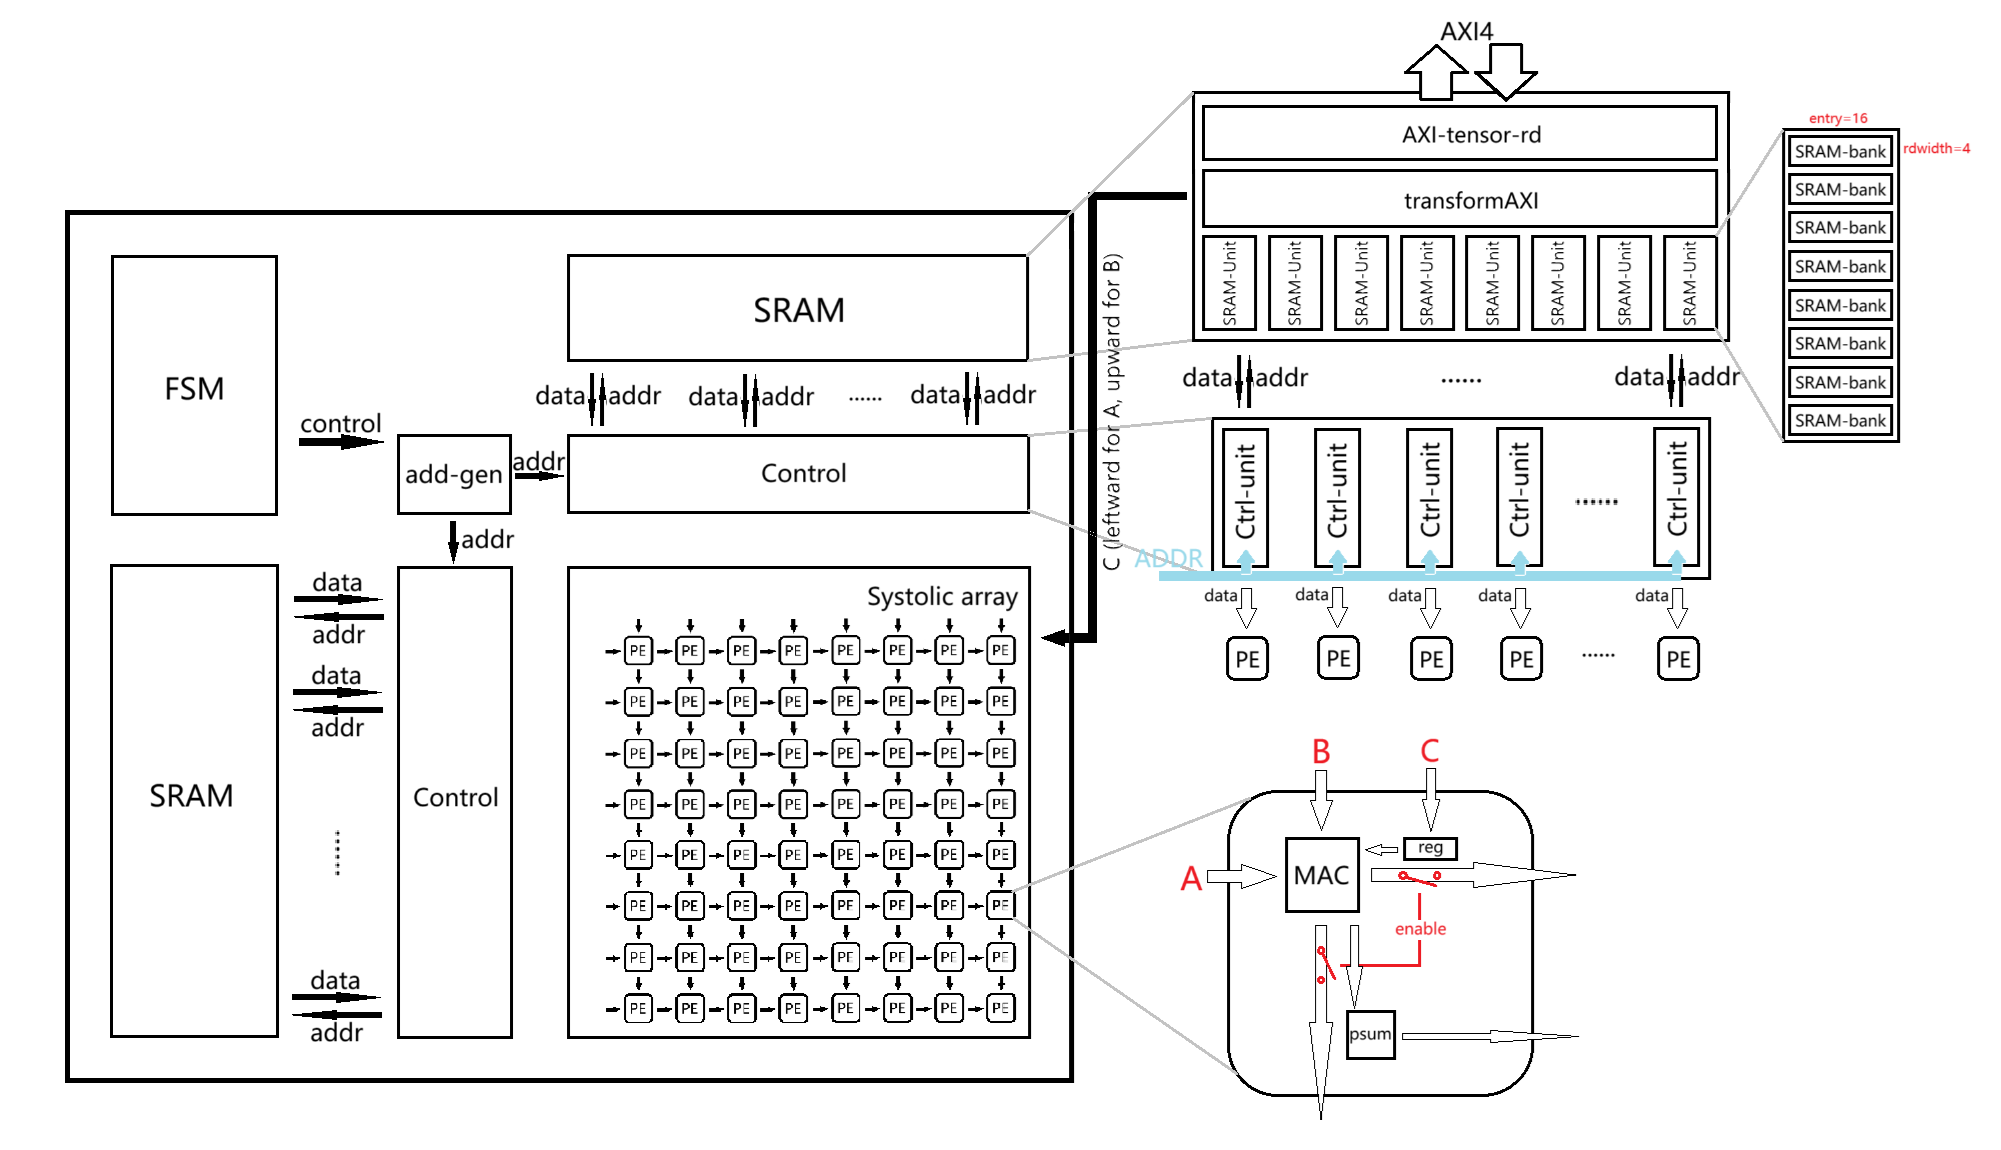
\includegraphics[width=0.4\textwidth]{架构.png}
      \caption{A/B/C 数据流向示意}
      \label{fig:sram-abc}
    \end{figure}
\subsection{整体架构}
\begin{itemize}
  \item transformAXI:将AXI传递的信号进行转换:针对A,B,C不同的类型进行不同的转换
  \item A传入了SRAMA,B传入了SRAMB,C传入了systolic(但是为了不造成布线密集,C一次只能向一个systolic传入32bit)
  \item addrgen.sv:生成取数的地址,在SRAMA,SRAMB中取数
  \item PE.sv单个的处理单元,systolic.sv:systolic array
\end{itemize}

\subsection{创新点}
\begin{itemize}
  \item 采用了分块乘法的方式,在最后阶段进行加法,提高并行性
  \item 每个PE可以支持1个FP16/FP32,浮点乘法采用pipeline形式,4个INT4,INT8的乘法,INT4,INT8复用了加法器,FP16/FP32复用了MAC
  \begin{figure}[H]
      \centering
      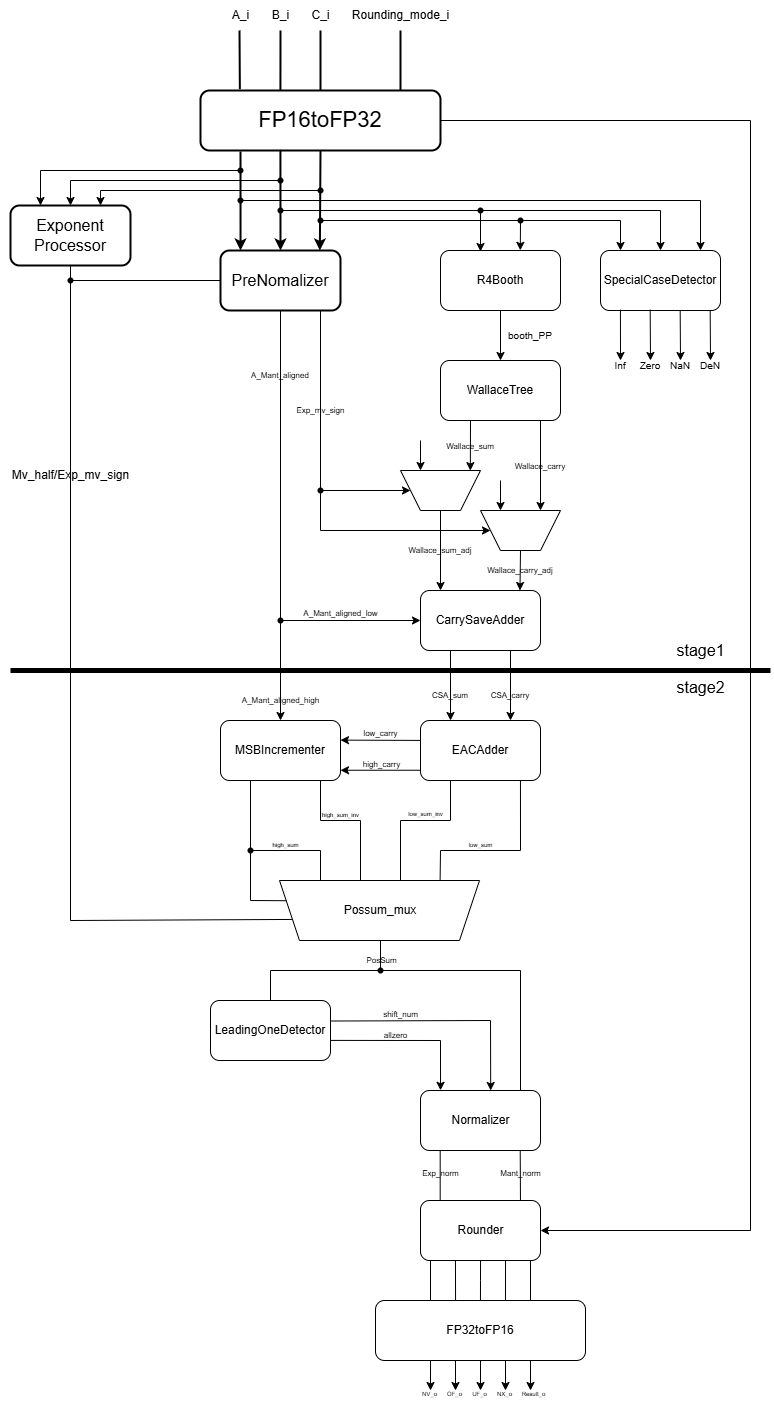
\includegraphics[width=0.4\textwidth]{FP.png}
      \caption{3种形状的运算}
      \label{fig:FP16/FP32}
    \end{figure}
  \item 新增addrgen与control模块,将复杂的逻辑与PE解耦合,使得PE仅需提供简单的功能
  \item 将所有的enable使能信号也完全变成systolic形式,从而不必关注PE内部各种判断与stall,PE完全接受外部使能信号
\end{itemize}

\subsection{计算方法}
\begin{figure}[H]
      \centering
      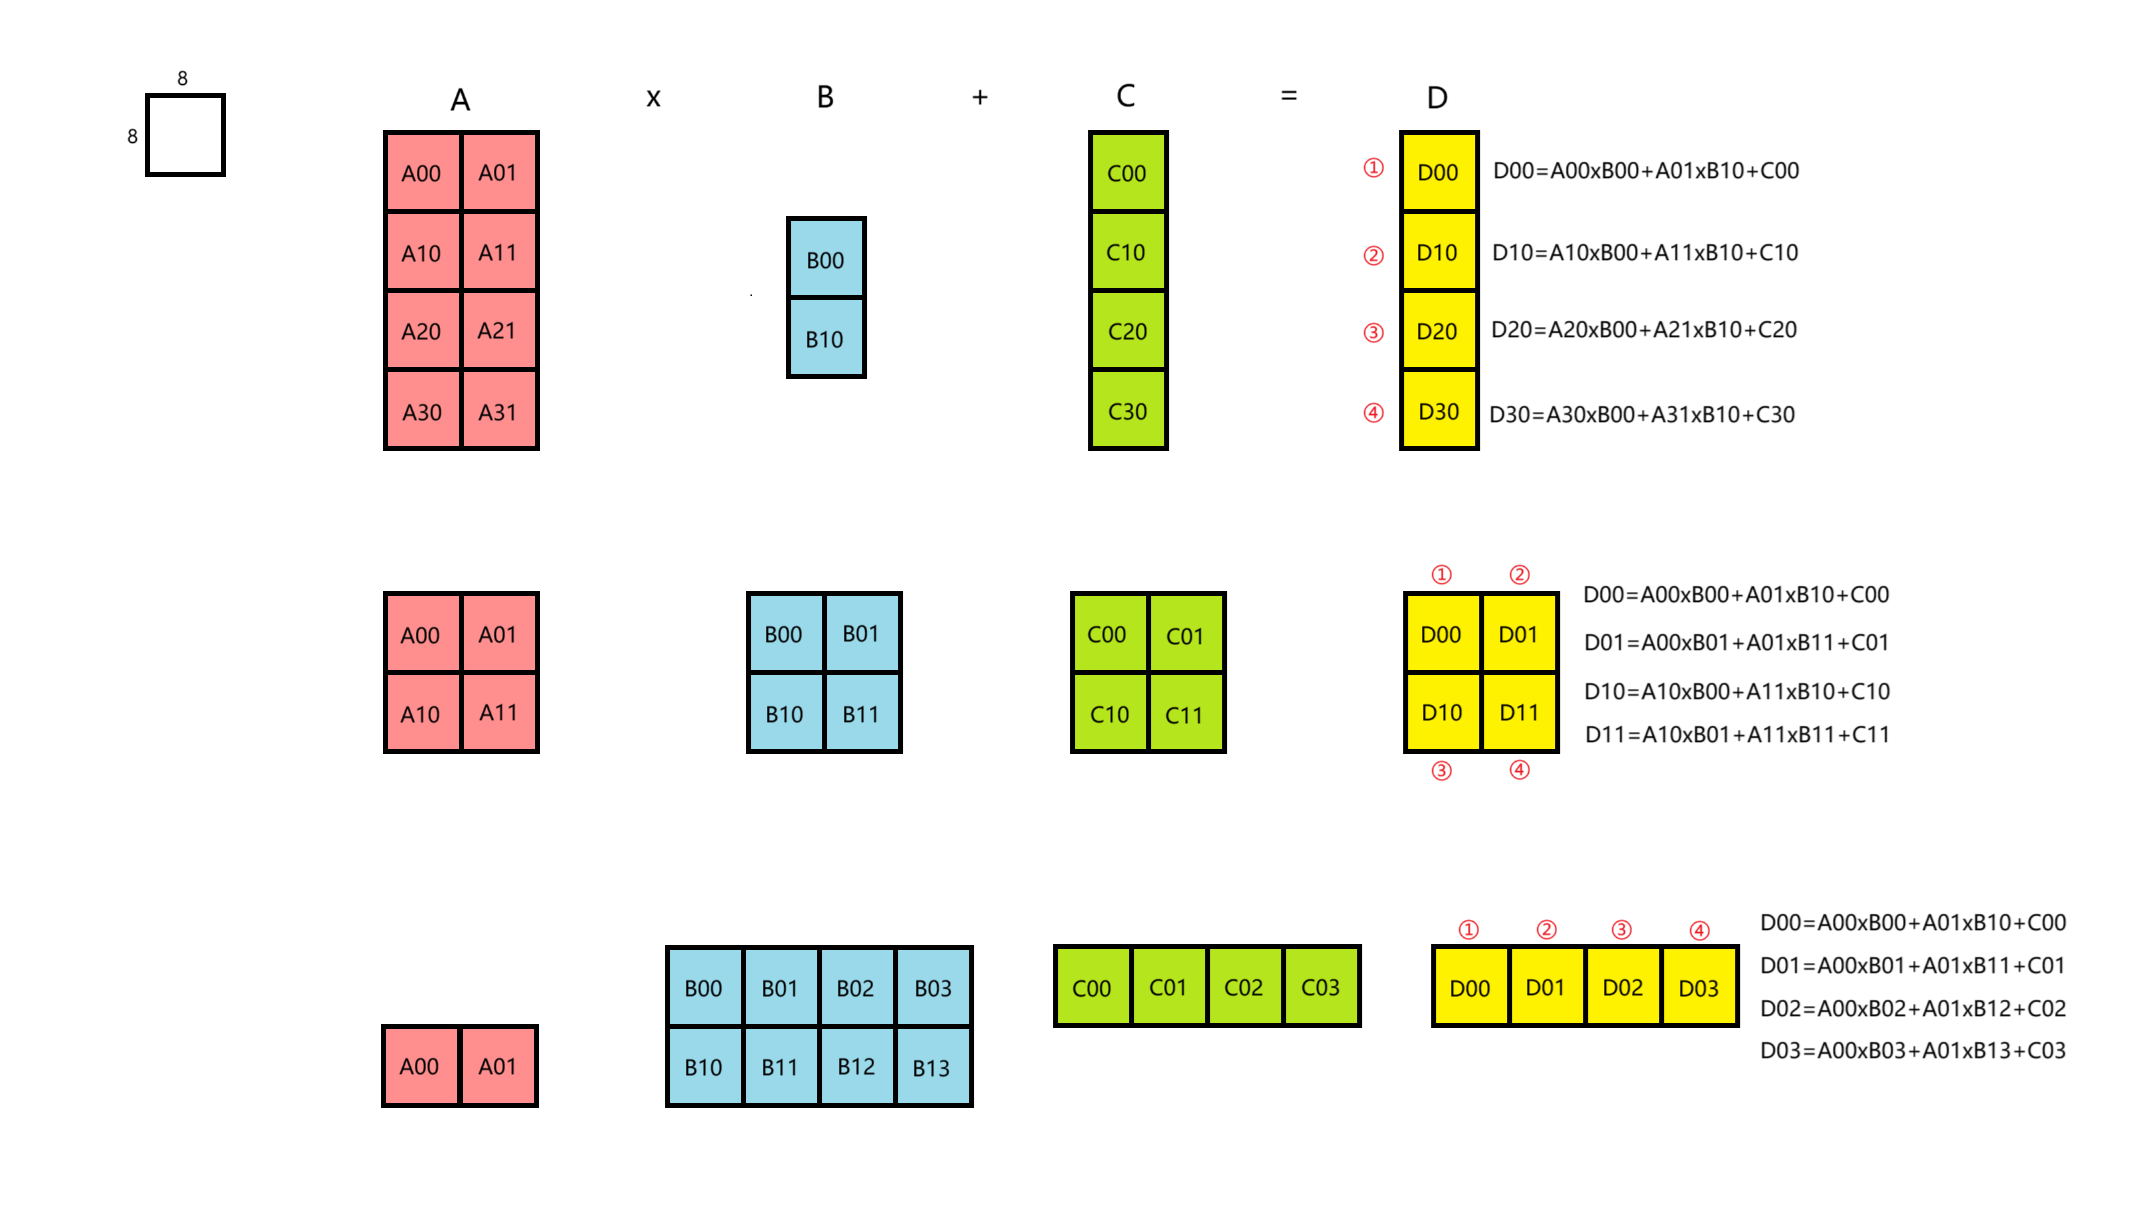
\includegraphics[width=0.4\textwidth]{计算.png}
      \caption{3种形状的运算}
      \label{fig:compute}
    \end{figure}
如图所示,这里的A,B,C中的每一块都是8*8的矩阵,从而对于D而言,一共四块,最后都存放在PE中的regfile上,
第一块的(0,0)存在regfile的31~0bit,第二块的(0,0)存在PE的63~32bit,依次类推


对于FP32,FP16而言,需要考虑的是两级流水,所以两次计算之间不能产生依赖,这些已经由addrgen完成取数的无关性
对于INT8,由于能一次算8个块乘法,因此需要在最终加入一个累加阶段,将regfile中的数进行累加,这里巧妙地运用了INT4
中最多每个结果只需要16bit,从而在regfile只有128bit的情况下,复用了资源同时存8个INT4乘累加的结果

\subsection{信号说明}
para\_pkg.sv:\\
data\_type: 0:FP32,1:FP16,2:INT4,3:INT8\\
compute\_shape: 计算的是哪种类型的乘法:0:M32K16N8,1:M16K16N16,2:M8K16N32\\
AXI\_in\_t:AXI需要传入tensorecore的信号,作为一个接口,我要构建tensorcore只关心这些信号\\
AXI\_out\_t:tensorcore需要传出到AXI的信号,作为一个接口,我要构建tensorcore只关心这些信号\\
其它重要信号在代码中有注释

transformAXI.sv:\\
传入了256bit(rdbus的带宽)的信号,现在需要将这些信号传递到SRAM(A,B)和systolic(C)中

addrgen.sv:\\
在从systolic array中接收到en后,开始进行计算,维护一个计数器counter,从而能够实现有规律的取数逻辑

control.sv:\\
在从内存中取出数字后,按照类型进行一定的重排/复制

sram.sv:\\
这里实现了两个SRAM(但我比较担心后面可能会被综合成寄存器)\\
SRAM\_A:由8个小SRAM组成,每个小SRAM由8个bank组成(每个bank4bit,刚好最低支持INT4),每个小SRAM作为对接PE的端口,其中写入逻辑用FIFO实现(不对外提供写地址),对于一个bank:要么写入32bit,要么不写\\
SRAM\_B:由8个小SRAM组成,每个小SRAM由8个bank组成(每个bank4bit,刚好最低支持INT4),每个小SRAM作为对接PE的端口,写入用FIFO,对于一个bank:要么写入4bit,要么不写

PE.sv:\\
作为一个PE,需要维护register\_pointer,指向需要写入的寄存器

ENABLE.sv:\\
实现了信号的systolic传输

\subsection{项目不足}
\begin{itemize}
    \item 目前我认为瓶颈主要在于取数带宽上,对于我的systolic与调度能提供高性能计算,在有多个SRAM取数从而隐藏传输延迟的情况下效果更佳
    \item 由于我限制了systolic中的每个PE每次传入C只能写入32bit,又由于AXI取数方式的约束,导致此时大大浪费了AXI的带宽(但是确实在一些情况下无法做到)
    \item 目前部分信号宽度太大,但是感觉综合工具应该能自动优化(纯粹是一开始没确定位宽)
    \item SRAM是存储资源最丰富的地方,目前来看可能很难综合成SRAM,而是会变成寄存器堆
\end{itemize}

\section{如何验证架构}
目前马晋已经完成了tensorcore本身的部分,想要验证,只需cd tensorcore/rtl/verilator,make run即可,
马晋配置了verilator环境,在tensorcore/.vscode/settings.json中
助教老师遇到任何关于tensorcore验证的问题都可以直接联系imagine(ma15807252614)
验证所写的文件在tensorcore/rtl/verilator/main.cpp中,助教老师可以用main.cpp的方式验证对于不同datatype和matrix shape的测试,只需要移除部分注释即可,
通过make run > out.txt,在out.txt中能看见输入矩阵,以及按照C++计算得到的输出结果以及按照tensorcore给出的输出结果。
\begin{figure}[H]
      \centering
      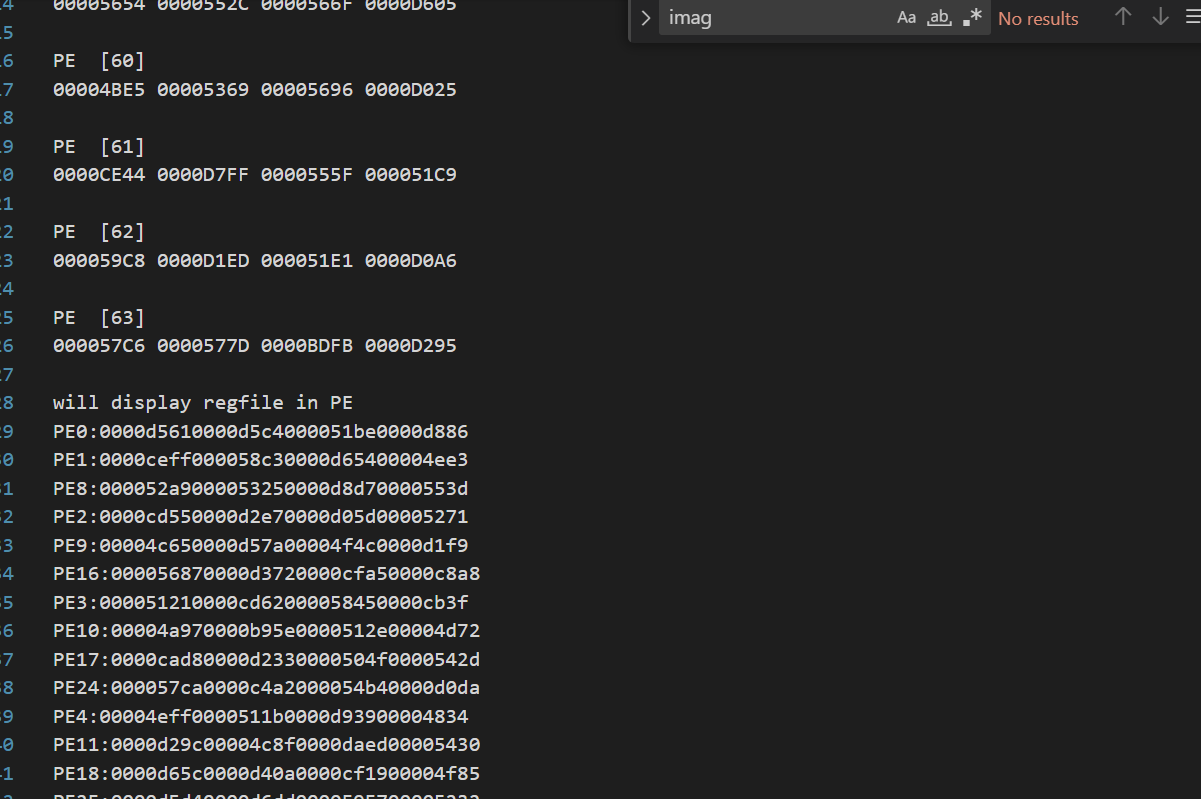
\includegraphics[width=0.4\textwidth]{image.png}
      \caption{输出结果}
      \label{fig:输出结果}
    \end{figure}
如图所示,will display前面的是用软件计算的结果,will display的是tensorcore输出的结果。
注意其中的mixed表示是否用混合精度训练,混合精度下的compute\_type与正常FP16相同,就是mixed信号置为1,
注意同时更改fmacase中的类型,混合精度为<half,half,float,float>,上面这四个分别对应于A,B,C,D的类型,如果是FP16,则为<half,half,half,half>,如果是INT4,则为<int4\_t,int4\_t,int4\_t,int>


\section{综合结果}
\begin{figure}[H]
      \centering
      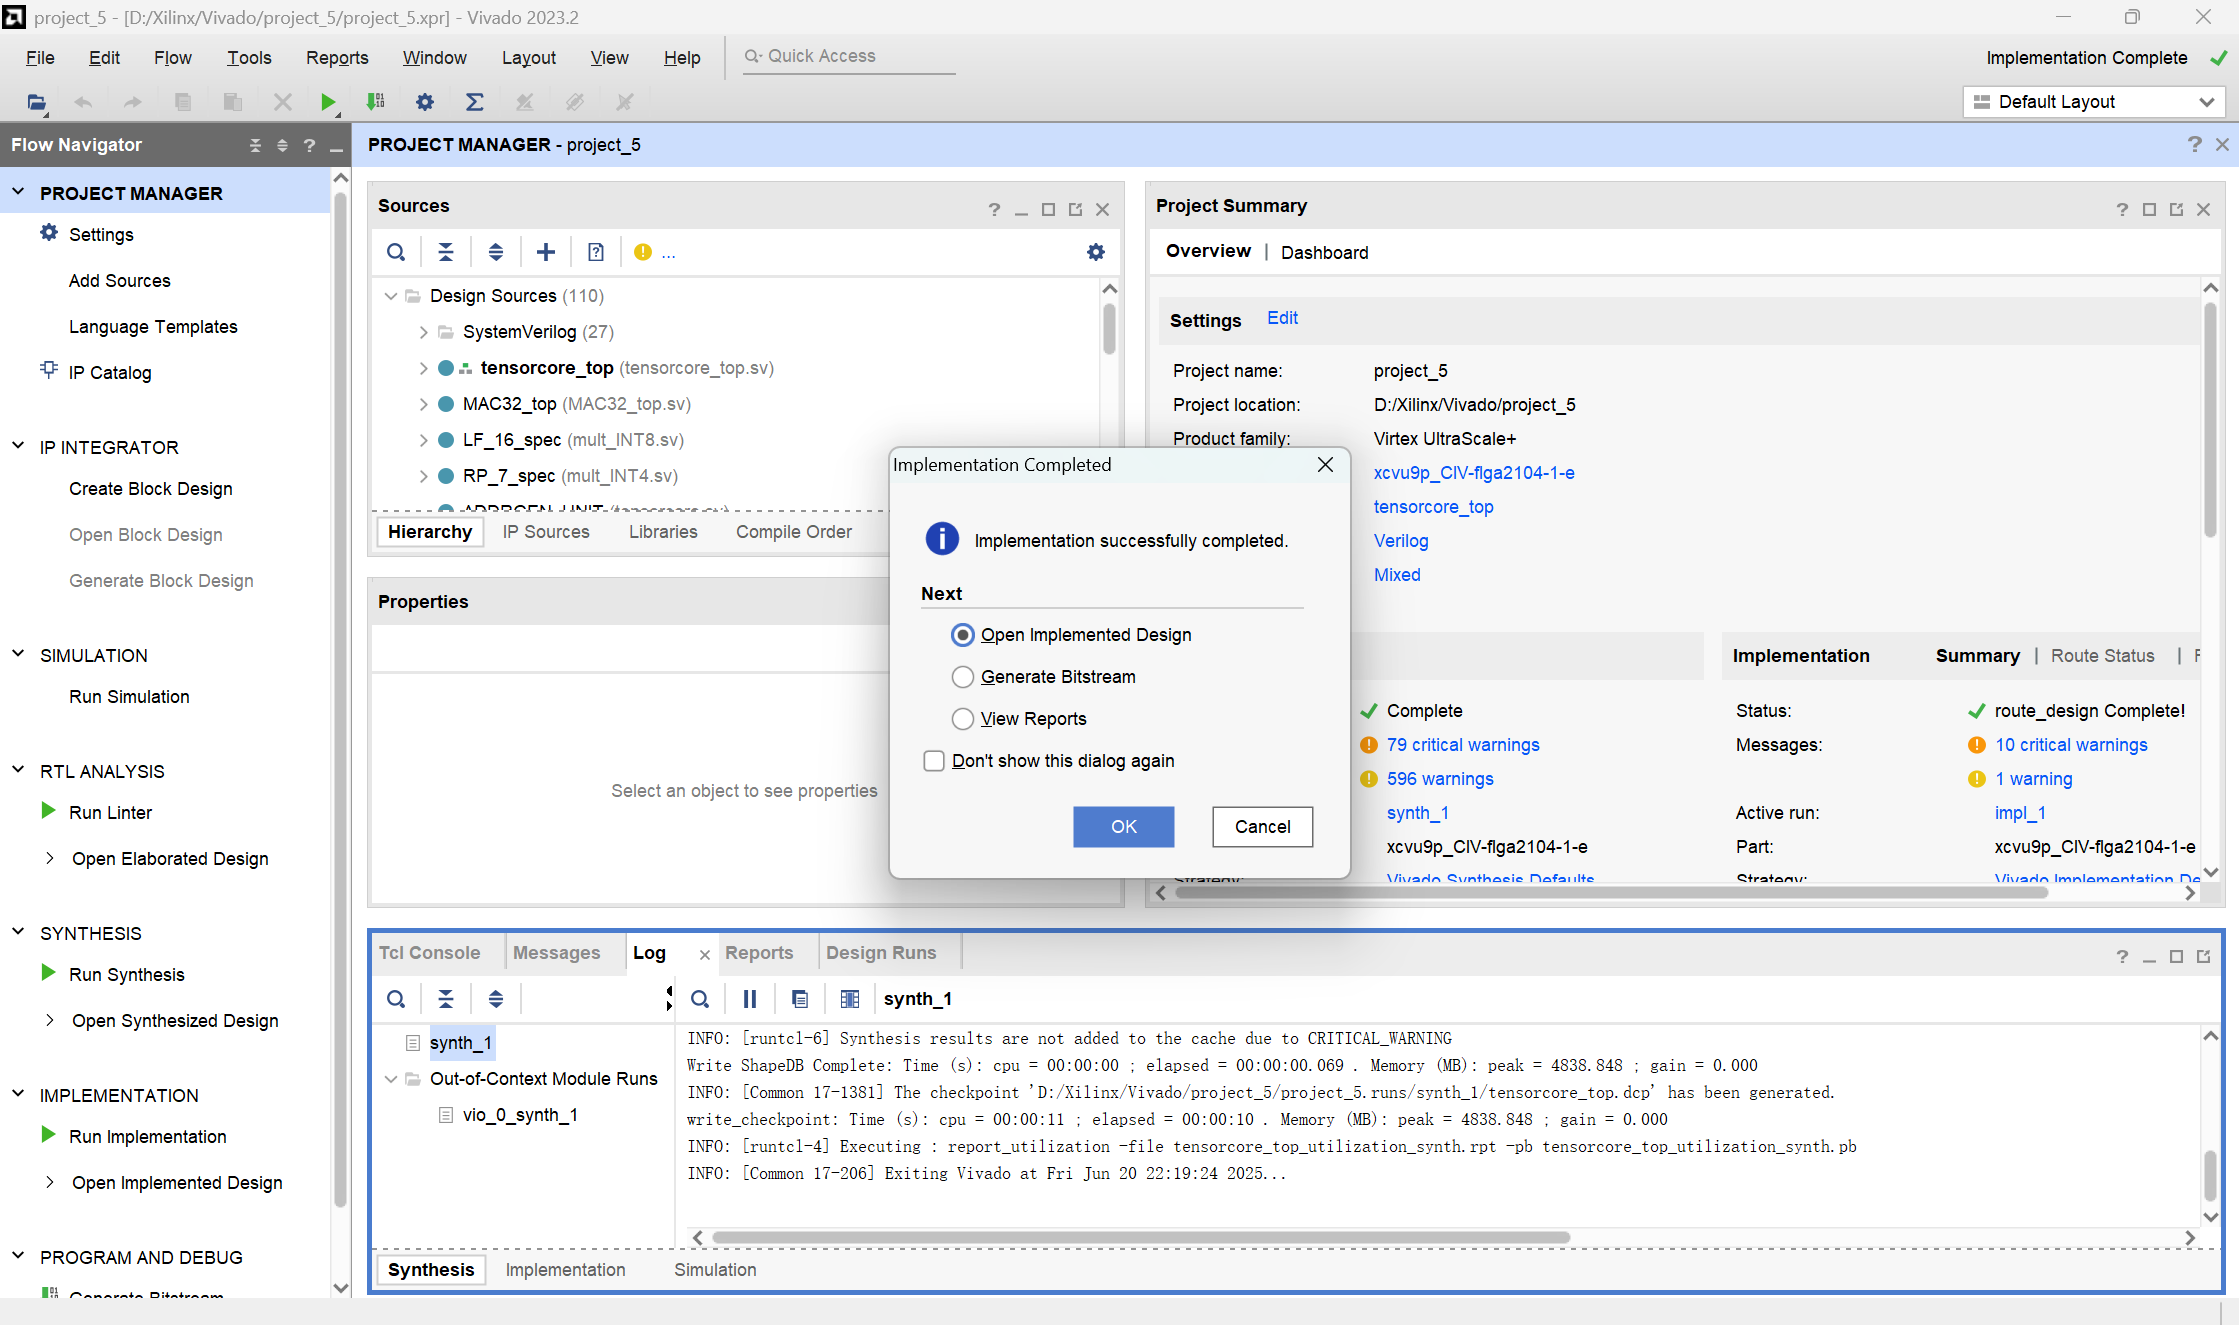
\includegraphics[width=0.4\textwidth]{布线.png}
      \caption{布线}
      \label{fig:布线}
    \end{figure}
\begin{figure}[H]
      \centering
      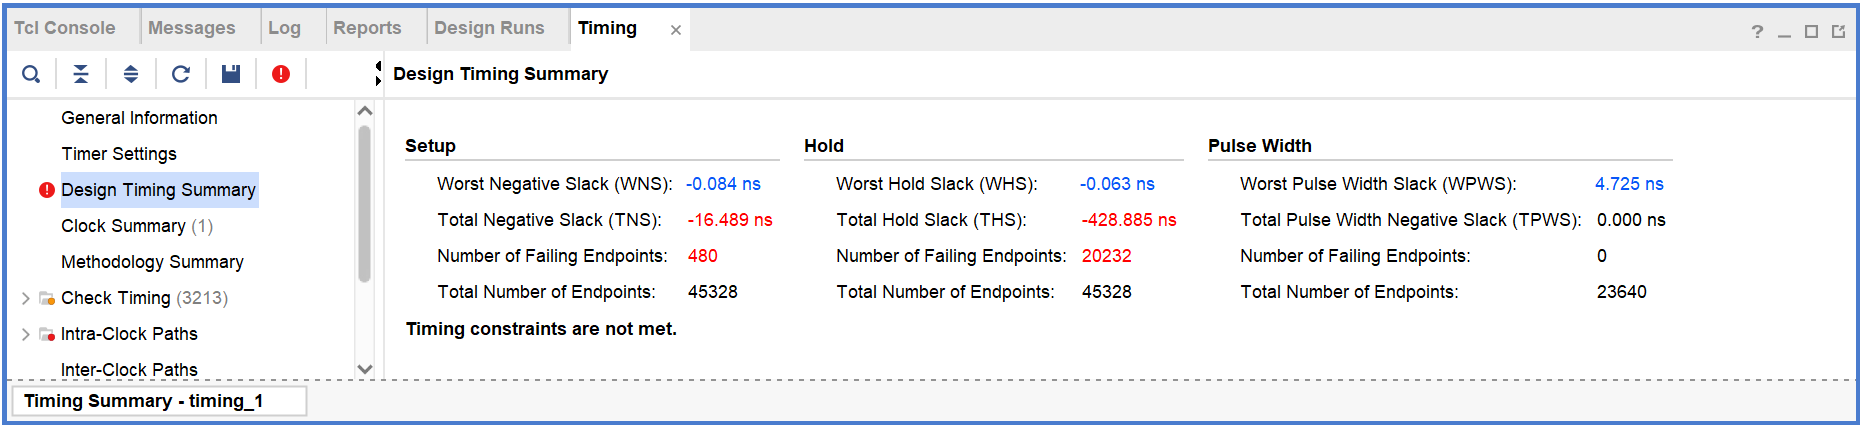
\includegraphics[width=0.4\textwidth]{综合100M.png}
      \caption{综合100M}
      \label{fig:综合100M}
    \end{figure}
\begin{figure}[H]
      \centering
      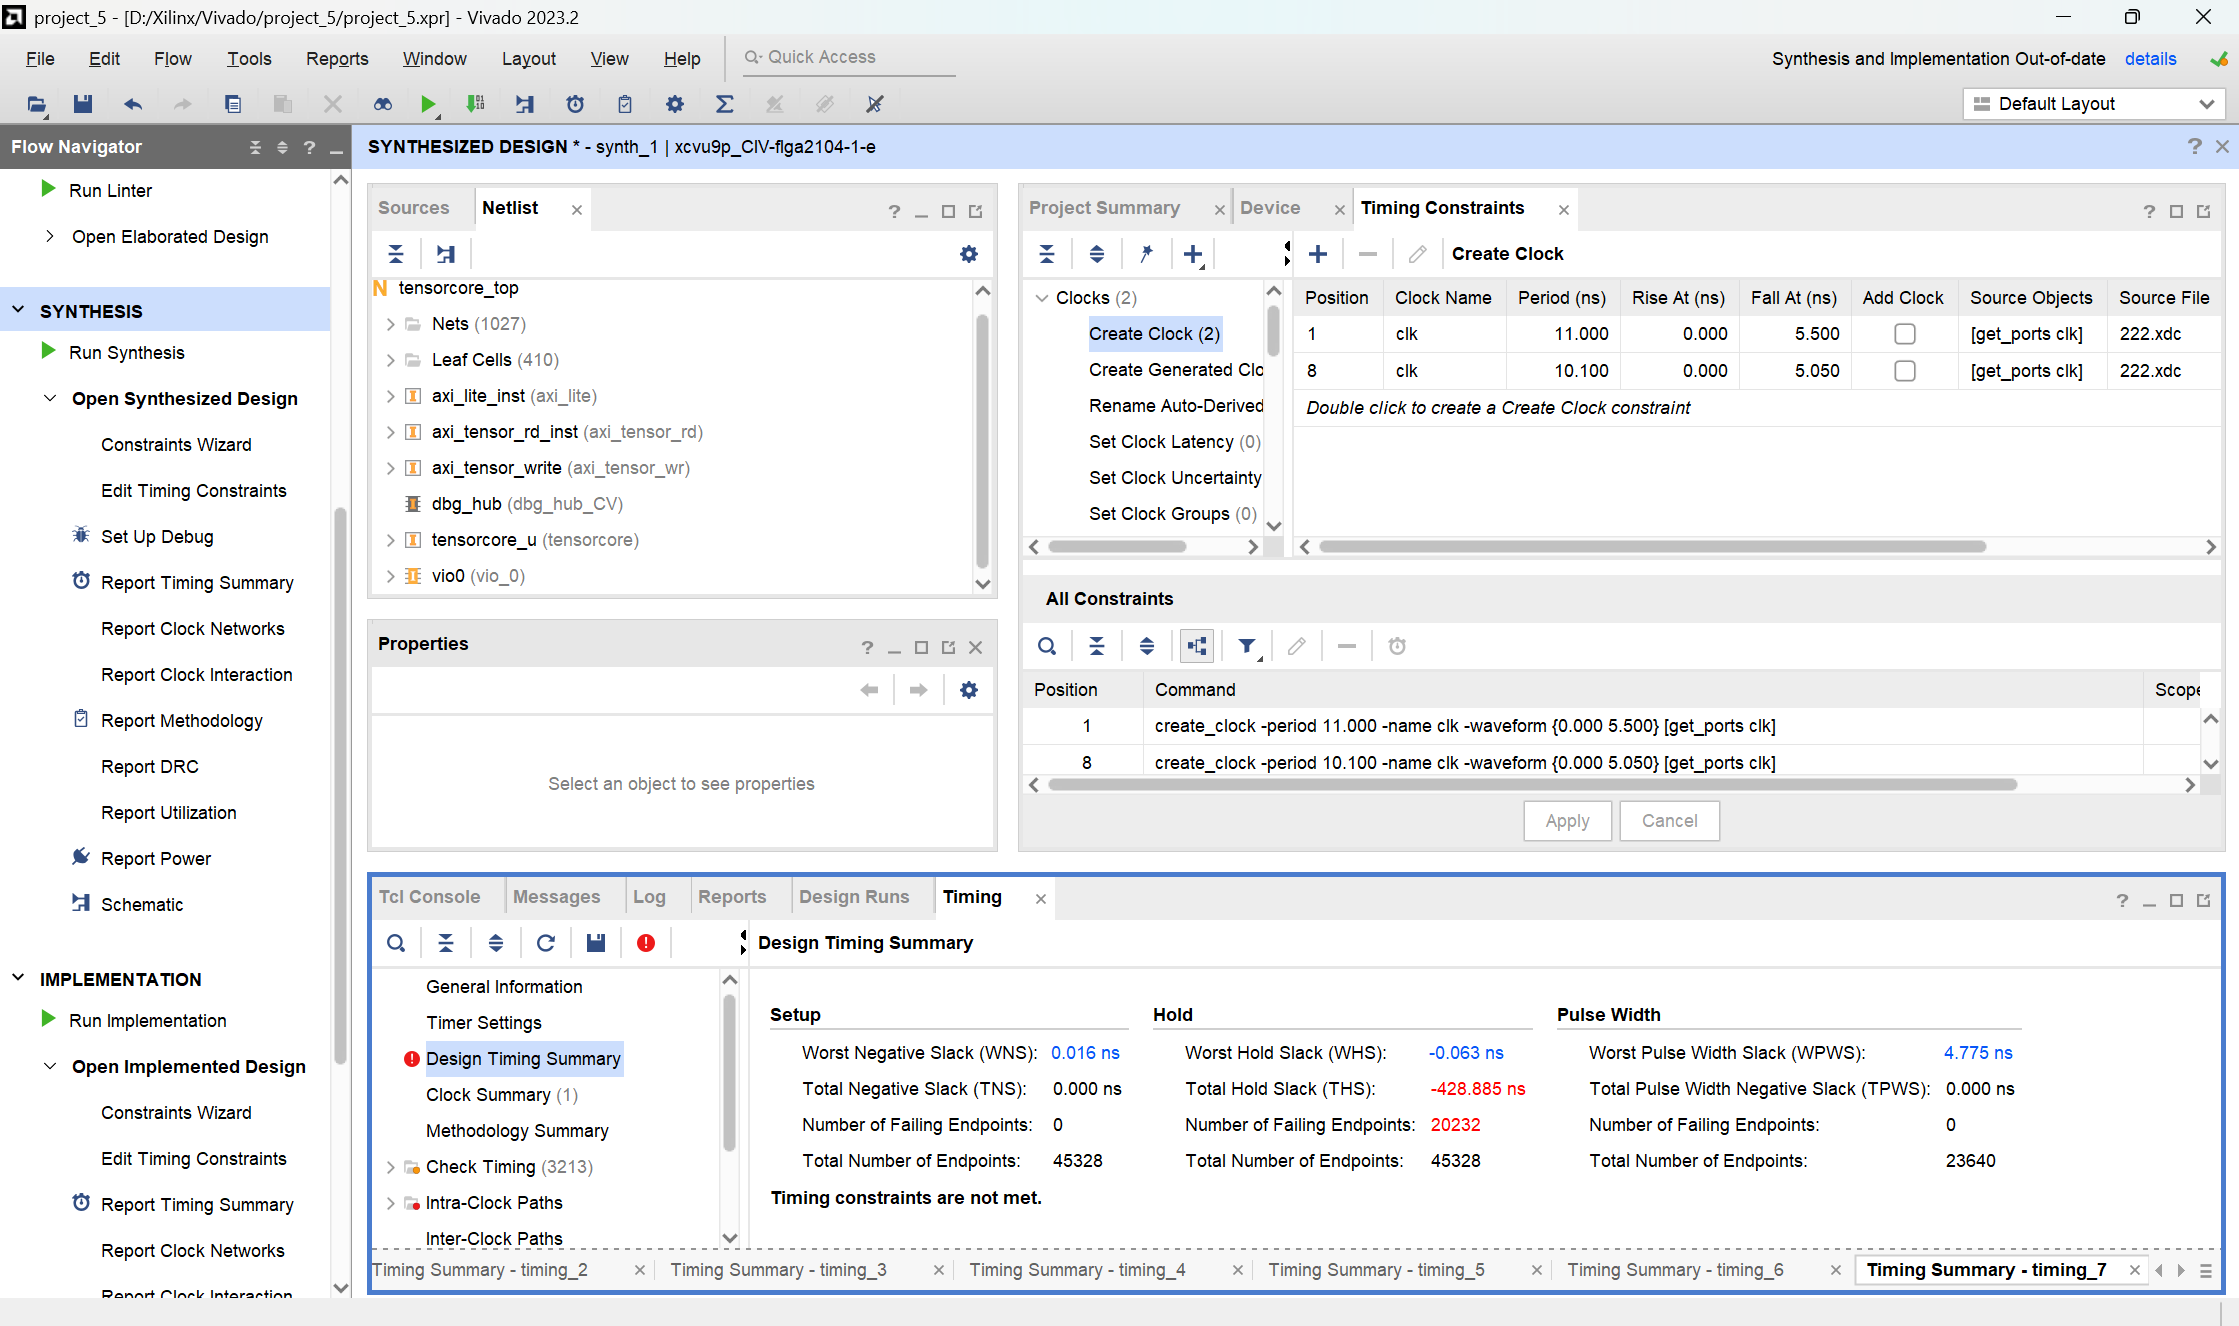
\includegraphics[width=0.4\textwidth]{综合99M.png}
      \caption{综合99M}
      \label{fig:综合99M}
    \end{figure}
\begin{figure}[H]
  \centering
  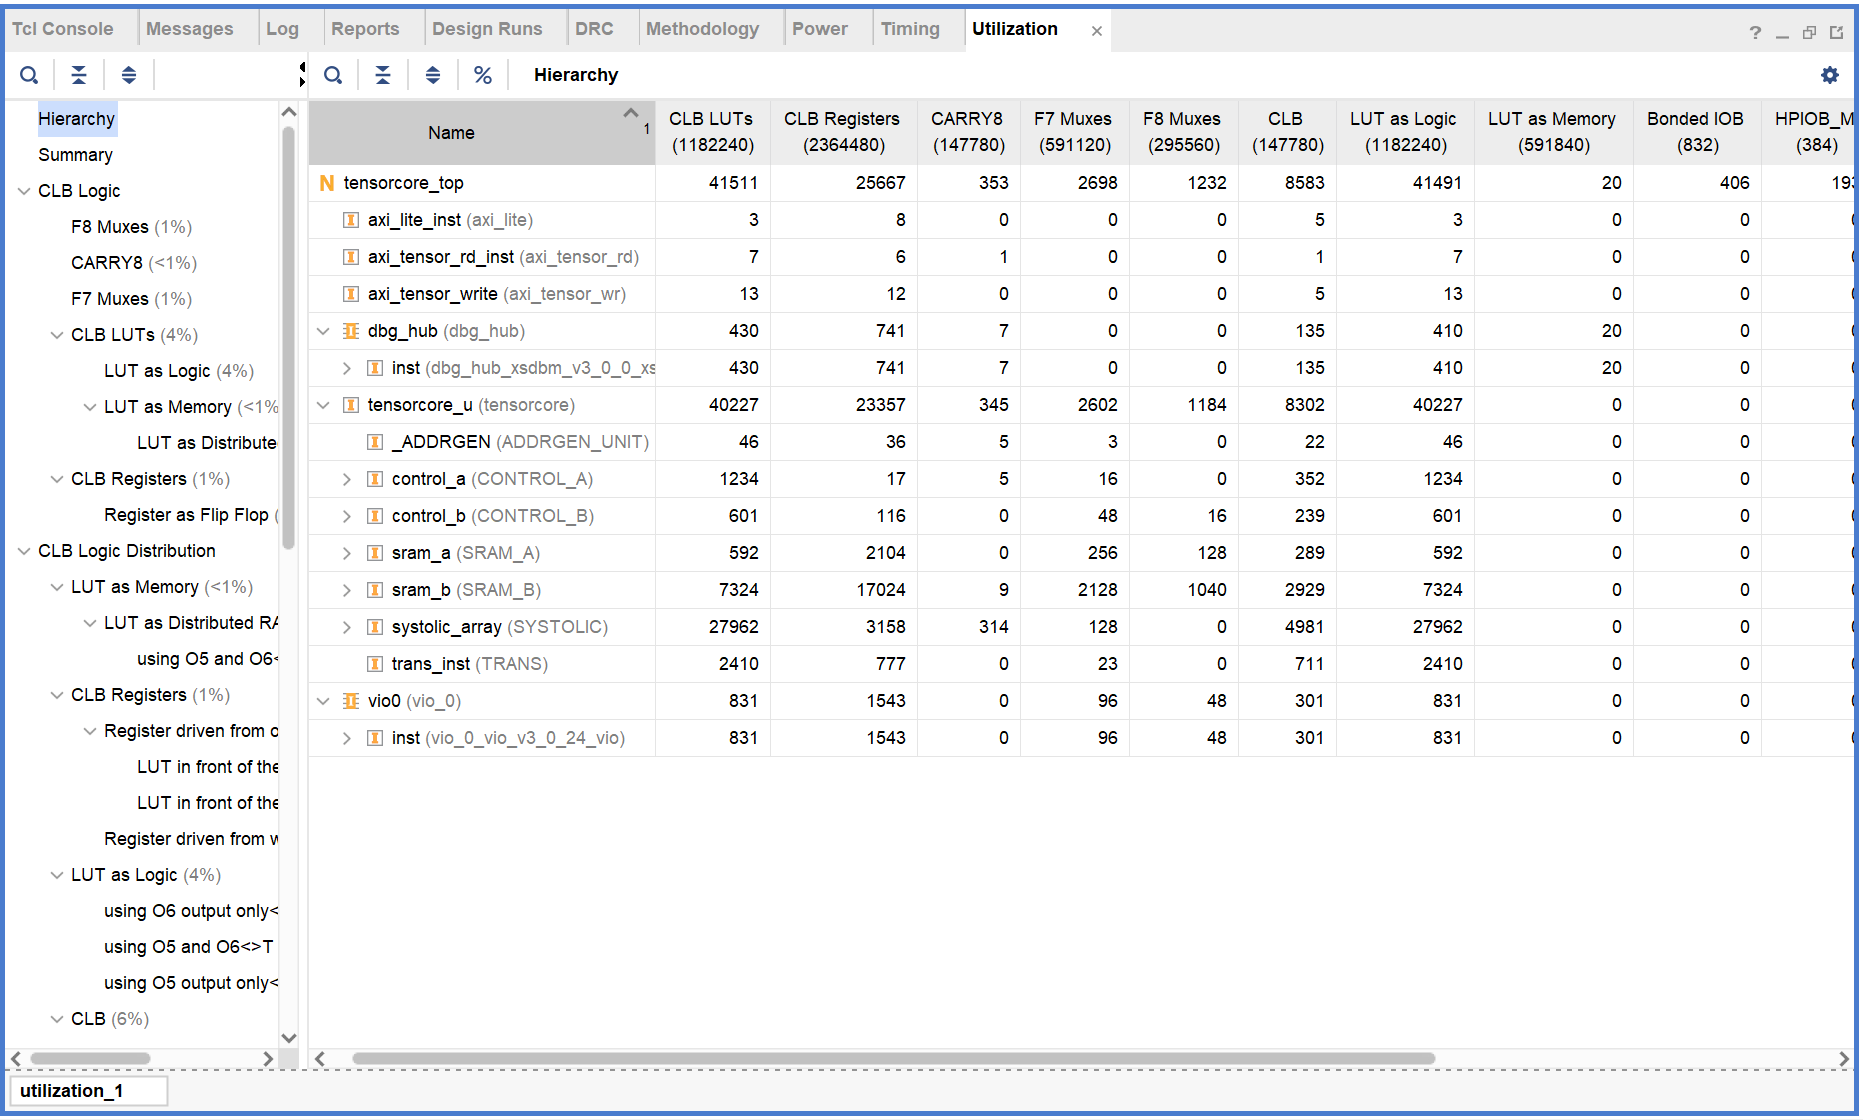
\includegraphics[width=0.4\textwidth]{资源.png}
  \caption{资源}
  \label{fig:资源}
\end{figure}
如图所示,经过测试,瓶颈在于PE只能达到100M(关键路径上),但是有一件感觉在综合中感觉逆天的事情是:
我尝试综合了PE中的MAC\_top.sv(为了结果准确,在现有的MAC\_top.sv输出加了一级寄存器),发现能达到远不止100M的频率,
但是PE.sv不知为何无法达到相应的频率,PE.sv中有很长的if-else,但我觉得这个路径相对于MAC\_top.sv中的乘加部分造成的延时应该微不足道。
总而言之,逆天PE触发的逆天机制是约束频率的罪魁祸首。



% 各模块
\section{分工}
分工主要是为了方便助教能了解每位同学负责什么,因此在查阅相应的部分没有完成或完善有问题的时候,可以去联系相应的同学
\subsection{马晋}
\begin{itemize}
  \item 完成了基本的MAC模块,并进行了二级流水(参考了多种版本FP的比较:排除了FPnew,因为FPnew冗余过多及实现简单,pipeline方式低效)
  \item MAC模块FP32的pipeline+MAC模块中的加法部分(同时支持4bit和8bit)+FP16toFP32.sv
  \item transformtoAXI.sv+addrgen.sv+systolic.sv+control.sv+ENABLE.sv+tensorcore.sv,从数据传入到数据写回
  \item 对整体的tensorcore进行了测试以及debug,包括找到部分MAC的错误
  \item 完成了tensorcore中burst\_num和burst\_size以及systolic\_time和waitwrite\_time的计算并加入
  \item 全局统筹项目(前期讨论,后期解答王俊涵综合的问题)
\end{itemize}
\subsection{李亚飞}
\begin{itemize}
    \item 完成了tensorcore中burst\_num和burst\_size以及systolic\_time和waitwrite\_time的计算并加入
    \item 完成了各种axi的逻辑
    \item 完成了FP16toFP32模块+FP32toFP16.sv从而组合出MAC\_FP
    \item 组装了MAC\_FP和MAC\_adder从而完成顶层MAC,同时支持多精度FP,INT
    \item 对整个MAC模块进行了测试以及debug
\end{itemize}
\subsection{王俊涵}
\begin{itemize}
    \item 完成了mult\_INT4(自写testbench),mult\_INT8(自写testbench),CLA(自写testbench),MAC(testbench由马晋提供)的验证
    \item 完成了MAC的综合+最终top的综合
\end{itemize}
\subsection{补充}
\begin{itemize}
    \item 马晋和李亚飞参与了初步的架构构建,在这个过程中马晋提出了采用分块乘法并在最后阶段做加法的想法,两人确定了其中部分参数
    \item 马晋自己完成了最终的架构构建:考虑了数据排布的影响,否决了前面提出的矩阵乘法的顺序
    \item 在最终的架构构建阶段,考虑将systolic与PE的复杂性解耦合,用addrgen专门生成数据取地址,大大提高了效率
    \item 马晋可能会考虑继续对于架构进行优化,目前在INT4与INT8的情况下,算力>>带宽,但是很容易将架构进行扩展,利用多个SRAM使得算力得到充分运用
\end{itemize}
\subsection{贡献度:仅供参考,并不准确}
\begin{itemize}
    \item 马晋: 72\%
    \item 李亚飞: 23\%
    \item 王俊涵: 5\%
\end{itemize}
\end{document}